\section{Realization}
%Focus generale sulle tecnologie utilizzate
In this section we outline the technical aspects concerning the realization of our framework. Therefore we first present the enabler technologies through which we instantiate the design principles presented in \cref{sec:design}. After that, we discuss the interaction workflow between the instantiated technologies. Finally, we show the implementation details.
\begin{figure}[t]
\centering
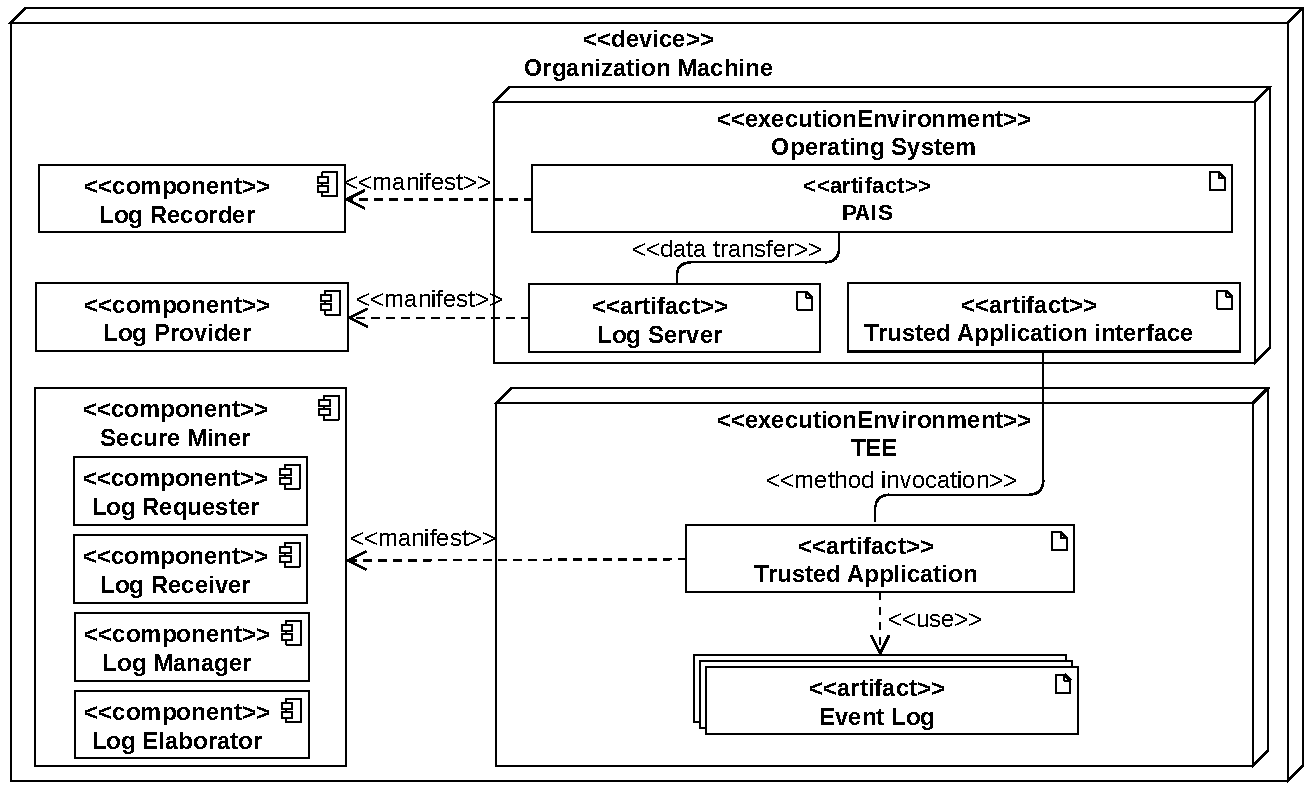
\includegraphics[width=12cm]{content/figures/deployment_diagram.pdf}
\caption{UML deployment diagram.}
\label{fig:deployment_diagram}
\end{figure}
\subsection{Deployment}
As follow, we bridge the gap between high-level system architecture and its practical realization. \cref{fig:deployment_diagram} depicts a \textit{UML deployment diagram} \cite{koch2002expressive} that aims to help with understanding the instantiated infrastrucuture. 

The \texttt{Organization Machine} represent the physical computation \textit{device} embracing the software and hardware entities of the company. The \texttt{Log Recorder}, the \texttt{Log Provider} and \texttt{Secure Miner} are included in the \texttt{Organization Machine} as abstract \textit{components} . These logical elements incorporate the core functionalities already discussed in \cref{sec:design}. The \texttt{Organization Machine} is characterized by two \textit{execution environment}s namely the \texttt{Operative System} and the \texttt{Trusted Execution Environment}.

Software elements that are exposed to the users of the \texttt{Organization Machine} run inside the \texttt{Operative System}. The functionalities offered by the 


%The \texttt{PAIS Interface} collects the logic to interact with the Process-aware Information Sytem (\texttt{PAIS}) of the \texttt{Organization}. \texttt{PAIS} systems help \texttt{Organization}s to handle business processes including accounting and resource management. The maintenance of event logs is the core tasks performed by these systems~\cite{Dumas.etal/2018:FundamentalsofBPM}. In our architecture, we generalize the interaction with \texttt{PAIS}s through the \texttt{PAIS Interface}. The \texttt{PAIS Interface} is queried by the local \texttt{Log Provider} for event logs to be fed into \texttt{Secure Miner}s.

\subsection{Workflow}
\subsection{Implementation}
%\subsubsection{Event Log Generation}
%Tecnologie utilizzate
%Sintesi del processo di generazione dei log
%\subsubsection{Trusted Miner and Log Provider}
%Tecnologia TEE usata
%Linguaggio usato per programmare in TEE
%Algoritmo implementato
%Rappresentazioni intermedie (PNML, Petrinet, ecc...)
%Linguaggio Log provider
